\subsection{Automatisation de la rééducation de la parole}

Une façon d'augmenter l'accessibilité de la rééducation de la parole 
--- et donc de mitiger les effets de l'aphasie de Broca ---
est de l'automatiser.
Un système automatique de rééducation n'a aucune contrainte temporelle.
Le nombre de séances par semaine n'est limité que par la disponibilité du patient,
plutôt que par le nombre d'orthophonistes disponibles.
Il élimine également le deuxième obstacle à l'accessibilité
en ramenant le coût du traitement à celui du matériel nécessaire.

Dans ce travail, nous proposons la création d'un système informatique 
pour la correction de la parole produite par une personne atteinte de l'aphasie de Broca.
Il s'agit d'une tâche assez commune dans le traitement orthophonique dispensé à ces patients%
~\cite{recover,Acharya_Wroten_2022}.
Le système doit être capable de transformer l'audio \(S_A\) (pour son aphasique) de la parole produite par le patient
en l'audio \(S_C\) (pour son corrigé) d'une parole correcte (voir la Figure~\ref{fig.global-system}).

\begin{figure}[hbt]
    \centering
    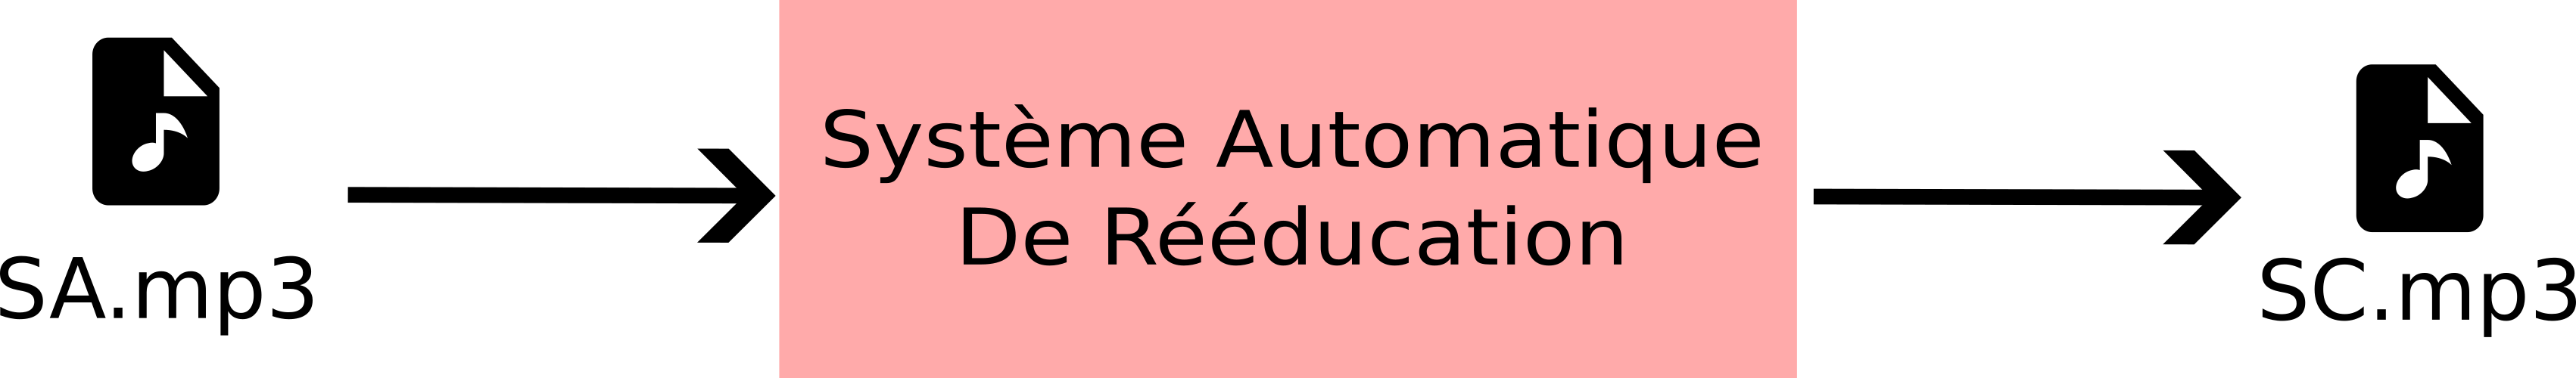
\includegraphics[width=.8\textwidth]{assets/images/system.png}
    \caption{Diagramme de fonctionnement du système proposé.}
    \label{fig.global-system}
\end{figure}
